\documentclass{ohm_project_description}

\projecttitle{Autonomous Paradrone}
\projectauthor{Labor für mobile Robotik}
\projectdate{2025}

\begin{document}

\maketitle
\thispagestyle{fancy}

\vspace*{-2.5cm}
\begin{figure}[h!]
    \centering
    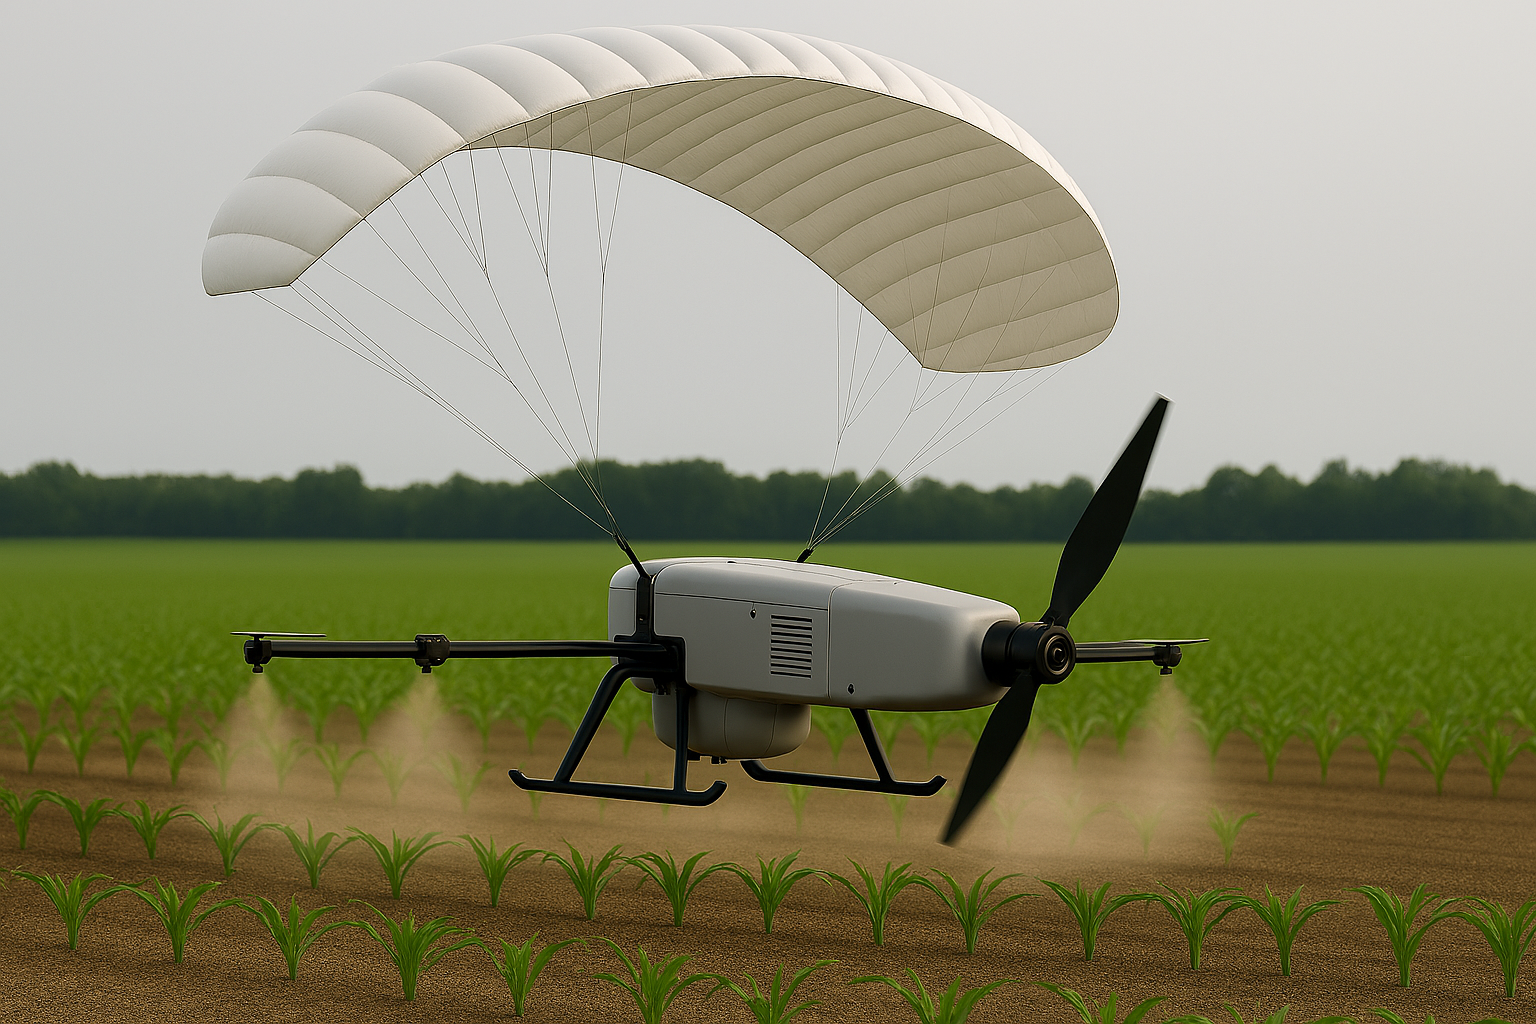
\includegraphics[height=4cm]{img/ParaDrone_2.png}
\end{figure} 


The goal of the project is the development of a small-scale prototype of a motorized paraglider drone (\emph{Paradrone}). The drone should be both remotely controllable and capable of autonomously flying a predefined route. For this purpose, it must be able to \emph{localize} itself in its surroundings, and a \emph{flight controller} must be developed. The hardware basis is an RC paraglider (approx. 1.5 m wingspan) which will need to be  equipped with an electric motor, battery, and a flight controller. \\

The work includes hardware development, software implementation, and the execution of flight tests in the drone laboratory of the Ohm Innovation Center (\emph{AerodrOhm}). 

\section*{Work Packages}
\begin{itemize}[leftmargin=0.5cm]
    \setlength\itemsep{.1em}
    \item Selection and adaptation of a suitable RC paraglider as the hardware basis
    \item Development of the flight controller and localization
    \item Validation of the flight controller in simulation
    \item Validation of the flight controller in flight tests
\end{itemize}

\section*{Requirements}
\begin{itemize}[leftmargin=0.5cm]
    \setlength\itemsep{.1em}
    \item Basic knowledge of a higher-level programming language (e.g., Python, C++)
    \item Experience with hardware development (e.g., microcontrollers, sensors, actuators)
    \item (optional) Basic knowledge of ROS (Robot Operating System)
\end{itemize}

\vspace{0.5cm}
This topic is ideally suited as a project work for two to three students. However, it can also be worked on in whole or in part as a Bachelor's or Master's thesis. 


\vfill
\textcolor{ohm_red}{\rule{\linewidth}{0.4mm}}
\textbf{\textcolor{ohm_red}{Labor für mobile Robotik}} \\
\begin{tabular}{@{}ll}
\textbf{Supervisor:} & Prof. Dr. Enrico Schröder \\
\textbf{E-Mail:}   & \href{mailto:enrico.schroeder@th-nuernberg.de}{enrico.schroeder@th-nuernberg.de} \\
\end{tabular}

\end{document}